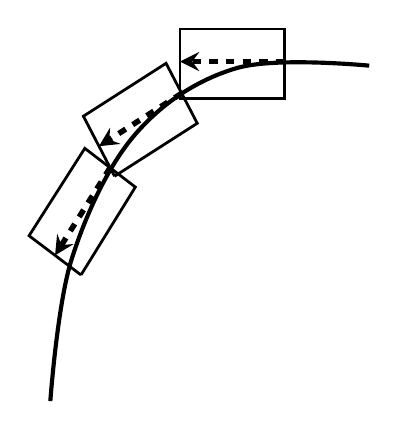
\begin{tikzpicture}[scale=6]
    % Include the PNG file as a background
    % \node[anchor=south west, inner sep=0] (image) at (0,0) {\includegraphics[width=10cm]{curve_rotation.png}};
    
    % Get the dimensions of the image
    % \begin{scope}[x={(image.south east)},y={(image.north west)}]
        % Example TikZ overlay:
        
        \draw[color=black, line width = 1.5] plot[smooth, tension = .6] coordinates{(.15, 0.1) (.195, 0.4) (0.33, 0.665) (0.545, 0.805)  (.825, .81)  }; 

        \draw[black, line width = 1] (.215,.367) -- (.33,.553) -- (.223,.635) -- (.105,.45) -- (.215,.367);
        \draw[black, line width = 1] (.286,.576) -- (.461,.688) -- (.395,.815) -- (.22,.703) -- (.286,.576);
        \draw[black, line width = 1]         (.4245,.74) -- (.645,.74) -- (.645,.8875) -- (.4245,.8875) -- cycle;
 %(.4245,.75) -- (.645,.75) -- (.645,.8975) -- (.4245,.8975) -- (.4245,.75);
        
        \draw[line width=2pt,black,-stealth, dashed] (0.2765, 0.594)--(0.16, 0.4085) node[anchor=south west]{};	
        \draw[line width=2pt,black,-stealth, dashed] (0.428, 0.7515)--(0.253, 0.6395) node[anchor=south west]{};	
        \draw[line width=2pt,black,-stealth, dashed] (0.645, 0.81875)--(0.4245, 0.81875) node[anchor=south west]{};	
        
    % \end{scope}
\end{tikzpicture}